\documentclass{beamer}
\hypersetup{colorlinks=true,urlcolor=blue,urlbordercolor=blue}
\usepackage[utf8]{inputenc}
\usepackage{graphicx}
\usepackage{amsmath,amssymb}
%Information to be included in the title page:
\title{Statistical Methods with Python}
%\author{Anonymous}
%\institute{Overleaf}
\date{}



\begin{document}
	
	\frame{\titlepage}
	
	\begin{frame}
		\frametitle{Curve fitting}
		Problem Statement:
		\begin{itemize}
			\item <1->Given some set of data points ($x$,$y$), we want to find the function $y(x)$ which most closely matches the data
		\end{itemize}
	\end{frame}

	\begin{frame}
		We want to go from this:
		\centering
		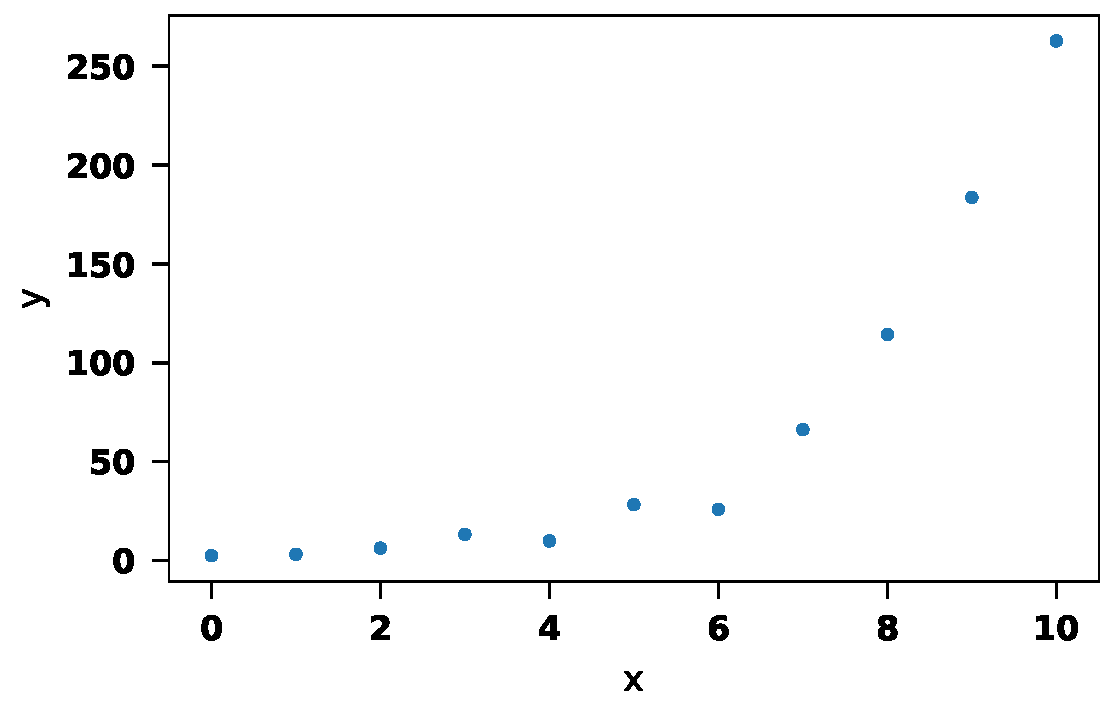
\includegraphics[width=10cm]{example_curve}
	\end{frame}

	\begin{frame}
		To this:
	\centering
	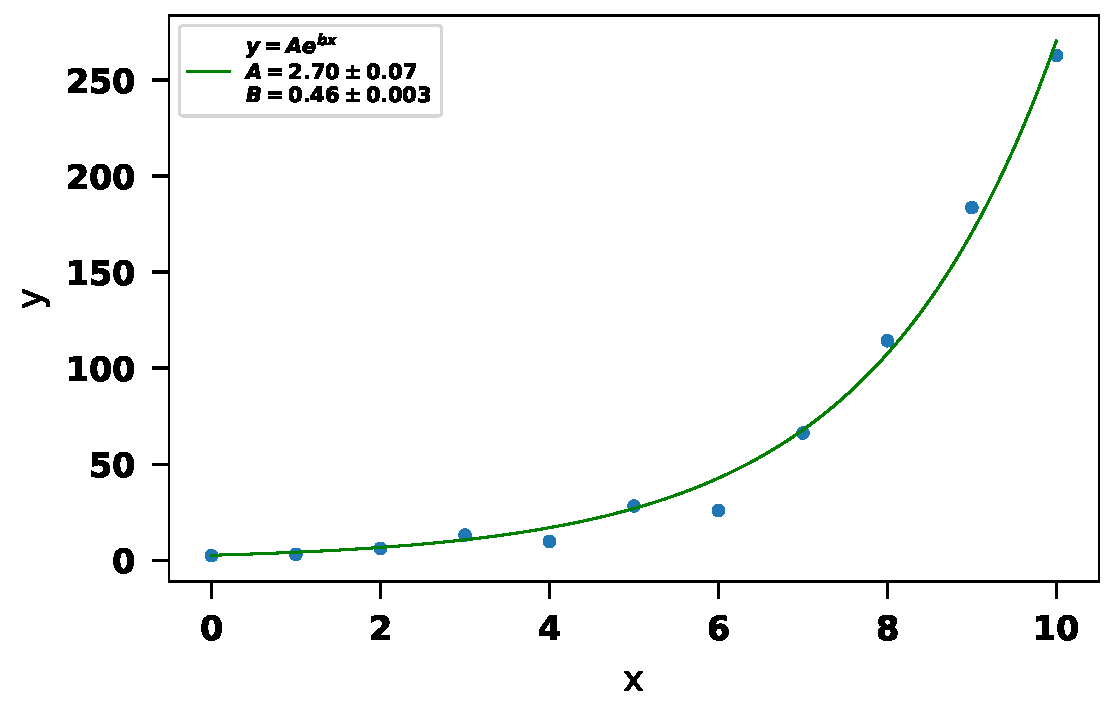
\includegraphics[width=10cm]{example_curve_fit}
	\end{frame}

	\begin{frame}
		\frametitle{Overall Procedure}
		Given a set of data, we must do a number of things to determine the so-called ``best-fit line''
		\begin{itemize}
			\item First, we must decide what \textit{type} of function to use
			\begin{itemize}
				\item Does my data look like a line ($y=ax+b$)? Does it look exponential ($y=ae^{bx}$)? Parabolic ($y=ax^2+bx+c$)?
			\end{itemize}
			\item <2->Having chosen a function, we need to find the values of the constants $a$, $b$, $c$ ... that cause the function to most closely match the data points
		\end{itemize}
	\end{frame}

	\begin{frame}
		\frametitle{Overall Procedure}
		Both of these items are complicated statistical problems that generally require a great deal of analysis
		\begin{itemize}
			\item Just because some function $y(x)$ ``looks like a good fit'' does not necessarily mean it is better than an alternative
			\begin{itemize}
				\item The more parameters in your function, the easier it will be to get a good looking fit.
				\item Comparing the ``goodness of fit'' of multiple functions requires an advanced understanding of statistics and probability theory; we will not get into that here
			\end{itemize}
		\item <2-> Bottom line: just because one function provides a better fit to the data does not mean that it is the statistically preferred function. A 5 degree polynomial will usually fit better than a simple exponential, but only because it has more ``degrees of freedom''
		\end{itemize}
	\end{frame}

	\begin{frame}
		\frametitle{Overall Procedure}
		Let's assume that you know which function you want to try and fit, and focus on how to actually find the best-fit values.
		\begin{itemize}
			\item <2-> This, too is a complicated question with many possible solutions depending on your needs
			\item <3-> I will introduce you to a popular algorithm and show you how to implement it in Python, just keep in mind there are many complementary ways of approaching this problem
		\end{itemize}
	\end{frame}

	\begin{frame}
		\frametitle{Revised Problem Statement}
		We have a set of data points $X$ and $Y$:
		\begin{align*}
			X &= x_1, x_2, x_3, \cdots, x_i, \cdots, x_n\\
			Y &= y_1, y_2, y_3, \cdots, y_i, \cdots, y_n
		\end{align*}
		We want to fit a function $f(x|{a, b, c, \cdots})$ to these data points\\
		
		(By this I mean a function $f(x)$ which depends on the parameters $a,b,c...$)
	\end{frame}

	\begin{frame}
		\frametitle{Example}
		\begin{center}
				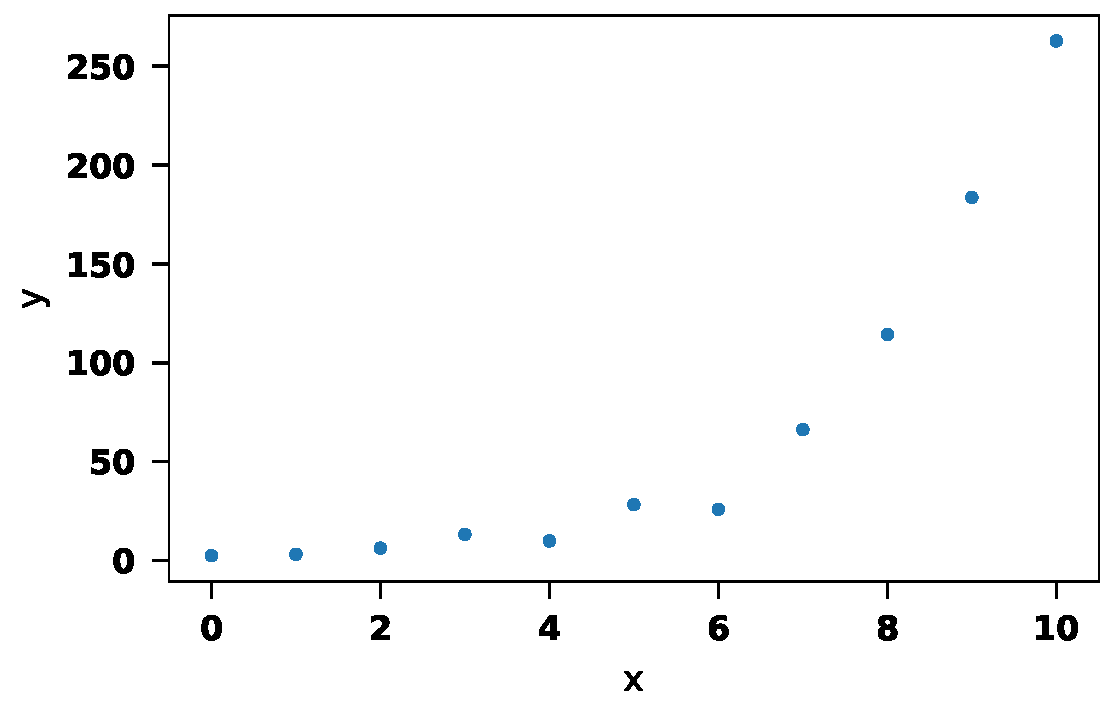
\includegraphics[width=6cm]{example_curve}
		\end{center}
		\small
		\begin{align*}
			X &= 0, 1, 2, 3, 4, 5, 6, 7, 8 ,9, 10\\
			Y &= 2.47,   3.18,   6.31,  13.24,   9.92,  28.32,  25.93,  66.25,
			114.29, 183.55, 262.68
		\end{align*}
		\normalsize
		\begin{equation*}
			f(x|{a, b, c, \cdots})=f(x|{a, b})=ae^{bx}
		\end{equation*}
	\end{frame}


	\begin{frame}
	\frametitle{Example}
	\small
	\begin{align*}
		X &= 0, 1, 2, 3, 4, 5, 6, 7, 8 ,9, 10\\
		Y &= 2.47,   3.18,   6.31,  13.24,   9.92,  28.32,  25.93,  66.25,
		114.29, 183.55, 262.68
	\end{align*}
	\normalsize
	\begin{equation*}
		f(x|{a, b, c, \cdots})=f(x|{a, b})=ae^{bx}
	\end{equation*}
	We want to choose the values of $a$ and $b$ that most closely match the data $X$ and $Y$
	\end{frame}

	\begin{frame}
		\frametitle{Finding the best fit curve}
		How do we define whether or not a line ``closely matches the data''?
		\begin{itemize}
			\item A \textit{perfect} fit would be one where every single data point lies exactly on top of the curve (the distance between each point and the curve is 0)
			\item < 2-> A curve which is farther away from the data points is a worse fit
			\item <3-> One easy way to determine how ``good'' the fit is: just sum the distance between points and line for every point. The smaller this number is, the better the overall fit.
		\end{itemize}
	\end{frame}






	\begin{frame}
		\frametitle{Fit Residuals}
		\begin{center}
			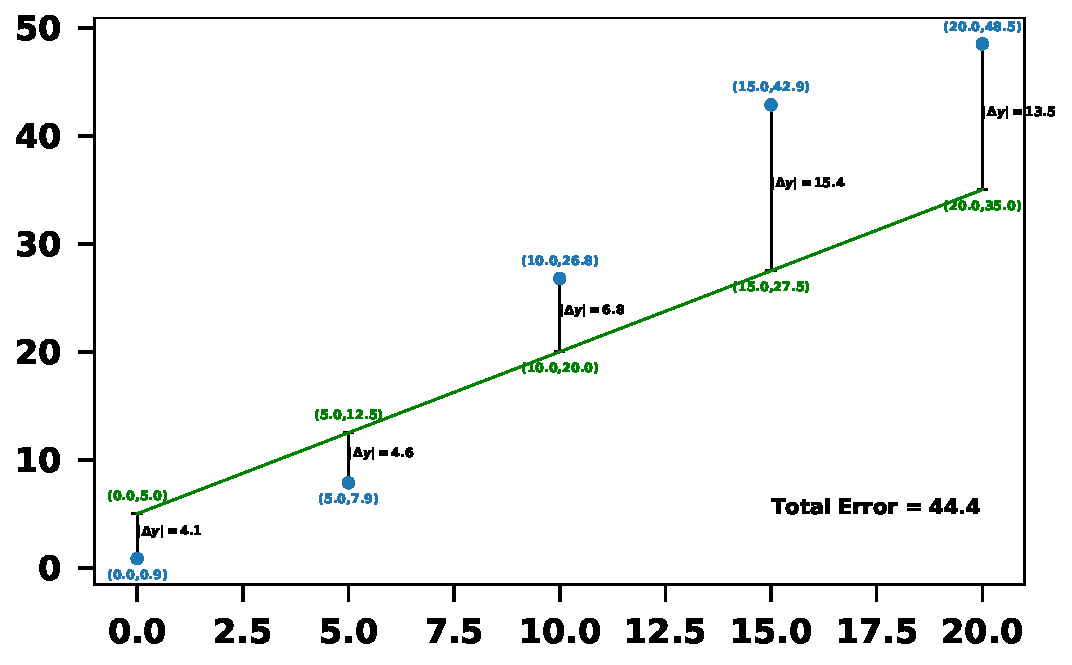
\includegraphics[width=10cm]{resid_visual}
		\end{center}
	\end{frame}






	\begin{frame}
		\frametitle{Fit Residuals}
		Each point has some error ($\Delta y$) which we usually refer to as the \textit{residual}.
		
		The \textit{total} residual $S$ is just the sum of the absolute value of each individual residual:
		\begin{equation*}
			S=|\Delta y_1| + |\Delta y_2| + \cdots + |\Delta y_n| = \sum_{i=1}^{n}|\Delta y_i|
		\end{equation*}

	\end{frame}






	\begin{frame}
		\frametitle{Fit Residuals}
	Each point has some error ($\Delta y$) which we usually refer to as the \textit{residual}.
	
	The \textit{total} residual $S$ is just the sum of the absolute value of each individual residual:
	\begin{equation*}
		S=|\Delta y_1| + |\Delta y_2| + \cdots + |\Delta y_n| = \sum_{i=1}^{n}|\Delta y_i|
	\end{equation*}
	\begin{itemize}
		\item  In practice, it's easier to sum the \textit{square} of the residuals, rather than their absolute values:
	\end{itemize}

	\begin{equation*}
		\mathbf{S\equiv\Delta y_1 ^2+ \Delta y_2^2+ \cdots + \Delta y_n^2 = \sum_{i=1}^{n}\Delta y_i^2}
	\end{equation*}
\end{frame}


	\begin{frame}
			\frametitle{Fit Residuals}
	\begin{equation*}
		S\equiv\Delta y_1 ^2+ \Delta y_2^2+ \cdots + \Delta y_n^2 = \sum_{i=1}^{n}\Delta y_i^2
	\end{equation*}
	Interpretation of $S$: the smaller the sum $S$ is, the closer the data points are to the curve\\
	The \textbf{optimal} function parameters $a$,$b$,$c$,... are those which \textit{minimize} $S$
	\begin{itemize}
		\item \href{https://phet.colorado.edu/sims/html/least-squares-regression/latest/least-squares-regression_en.html}{click here for visualization}
	\end{itemize}
	We can write a program to minimize $S$, or (in some cases) use calculus to minimize it by hand
	\end{frame}

\begin{frame}
	\frametitle{The Method of Least Squares}
	This method for finding the optimal parameters for the fitted function is known as the method of least squares, since it minimizes the sum of the square of the residuals
\end{frame}

\begin{frame}
	\frametitle{Procedure}
			We have a set of data points $X$ and $Y$:
	\begin{align*}
		X &= x_1, x_2, x_3, \cdots, x_i, \cdots, x_n\\
		Y &= y_1, y_2, y_3, \cdots, y_i, \cdots, y_n
	\end{align*}
	Function is $f(x|{a, b, c, \cdots})$
\end{frame}

\begin{frame}
	\frametitle{Procedure}
	We have a set of data points $X$ and $Y$:
	\begin{align*}
		X &= x_1, x_2, x_3, \cdots, x_i, \cdots, x_n\\
		Y &= y_1, y_2, y_3, \cdots, y_i, \cdots, y_n
	\end{align*}
	Function is $f(x|{a, b, c, \cdots})$\\
	\begin{equation*}
		S = \sum_{i=1}^{n}\left(Y_i-f(X_i)\right)^2
	\end{equation*}
\end{frame}

\begin{frame}
	\frametitle{Procedure}
	We have a set of data points $X$ and $Y$:
	\begin{align*}
		X &= x_1, x_2, x_3, \cdots, x_i, \cdots, x_n\\
		Y &= y_1, y_2, y_3, \cdots, y_i, \cdots, y_n
	\end{align*}
	Function is $f(x|{a, b, c, \cdots})$\\
	\begin{equation*}
		S = \sum_{i=1}^{n}\left(Y_i-f(X_i)\right)^2
	\end{equation*}
	The optimal set of parameters $a, b, c, \cdots$ are given by:
	\begin{align*}
		\frac{\partial S}{\partial a}&=0\\
		\frac{\partial S}{\partial b}&=0\\
		\frac{\partial S}{\partial c}&=0\\
		\cdots
	\end{align*}
\end{frame}



\begin{frame}
	\frametitle{Special Example: Linear best fit}
	We have a set of data points $X$ and $Y$:
	\begin{align*}
		X &= x_1, x_2, x_3, \cdots, x_i, \cdots, x_n\\
		Y &= y_1, y_2, y_3, \cdots, y_i, \cdots, y_n
	\end{align*}
	\begin{equation*}
		f(x|{a, b})=ax+b
	\end{equation*}
	\begin{align*}
		S &= \left((aX_1+b)-Y_1\right)^2+\left((aX_2+b)-Y_2\right)^2+\cdots\\
		S &= \sum_{i=1}^{n}\left((aX_i+b)-Y_i\right)^2
	\end{align*}
\end{frame}


\begin{frame}
	\frametitle{Special Example: Linear best fit}
	\begin{align*}
		S &= \sum_{i=1}^{n}\left((aX_i+b)-Y_i\right)^2
	\end{align*}
	\small
	\begin{align*}
		\frac{\partial S}{\partial a}=0&\implies \sum_{i=1}^{n}2X_i\left((aX_i+b)-Y_i\right)=\sum_{i=1}^{n}2\left((aX_i^2+bX_i)-X_iY_i\right)=0\\
		\frac{\partial S}{\partial b}=0&\implies \sum_{i=1}^{n}\left((aX_i+b)-Y_i\right)=nb+a\sum_{i=1}^{n}X_i-\sum_{i=1}^{n}Y_i=0\\
		&\left(nb+a\sum_{i=1}^{n}X_i-\sum_{i=1}^{n}Y_i=0\right)\div n\rightarrow b+a\bar{X}-\bar{Y}=0
	\end{align*}
	$\bar{X}$ and $\bar{Y}$ are the \textit{average values} of $X$ and $Y$:
	\begin{align*}
		\bar{X}&=\frac{1}{n}\sum_{i=1}^{n}X_i\\
		\bar{Y}&=\frac{1}{n}\sum_{i=1}^{n}Y_i
	\end{align*}
\end{frame}
\begin{frame}
	\frametitle{Special Example: Linear best fit}
	Now we have two equations, and two unknowns ($a$ and $b$) 
	\begin{align}
		\sum_{i=1}^{n}(aX_i^2+bX_i)-X_iY_i&=0\\
		b+a\bar{X}-\bar{Y}&=0
	\end{align}
\end{frame}


\begin{frame}
	\frametitle{Special Example: Linear best fit}
	I'll skip over the rest of the algebra to the final result:
	\begin{align*}
		a&=\frac{\sum_{i=1}^{n}\left(X_i-\bar{X}\right)\left(Y_i-\bar{Y}\right)}{\sum_{i=1}^{n}\left(X_i-\bar{X}\right)^2}\\ \\
		b&=\bar{Y}-a\bar{X}
	\end{align*}
\end{frame}





\begin{frame}{The General Case}
	In general, it is difficult/impossible to minimize $S=\sum_{i=1}^{n}\left(Y_i-f(X_i)\right)^2$ analytically\\ \vspace{1cm}
	We instead need to find a numerical approximation for the minimum
\end{frame}


\begin{frame}{The General Case}
	If the function $f=f(x|a,b,c,\cdots)$, the the sum $S$
	\begin{equation*}
		S=S(a,b,c,\cdots)=\sum_{i=1}^{n}\left(Y_i-f(X_i|a,b,c,\cdots)\right)^2
	\end{equation*}
	Is a function of the parameters $a,b,c,\cdots$ 
\end{frame}



\begin{frame}{The General Case}
	If the function $f=f(x|a,b,c,\cdots)$, the the sum $S$
	\begin{equation*}
		S=S(a,b,c,\cdots)=\sum_{i=1}^{n}\left(Y_i-f(X_i|a,b,c,\cdots)\right)^2
	\end{equation*}
	Is a function of the parameters $a,b,c,\cdots$ \\
	All that remains is to find the parameters $a,b,c,\cdots$ for which $S(a,b,c,\cdots)$ is minimal
\end{frame}



\begin{frame}{Minimizing $S$}
	In principle, this is just a matter of looping over all possible values of $a,b,c,\cdots$:\\
	for $a$ in range($a_i$,$a_f$,$\Delta a$):\\
	\hspace{.5cm}for $b$ in range($b_i$,$b_f$,$\Delta b$):\\
	\hspace{1cm}for $c$ in range($c_i$,$c_f$,$\Delta c$):\\
	\hspace{1.5cm}$\vdots$\\
	\hspace{2cm}$\cdots$ $s = S(a,b,c,\ldots)$
\end{frame}



\begin{frame}{Minimizing $S$}
	In principle, this is just a matter of looping over all possible values of $a,b,c,\cdots$:\\
	for $a$ in range($a_i$,$a_f$,$\Delta a$):\\
	
	This is rarely a practical solution: the total number of iterations is:
	\begin{equation*}
		N=\left(\frac{a_f-a_i}{\Delta a}\right)\left(\frac{b_f-b_i}{\Delta b}\right)\left(\frac{c_f-c_i}{\Delta c}\right)\ldots
	\end{equation*}
	So, even for a conservative precision $\Delta a=\Delta b=\Delta c=\ldots\approx 0.01$, you need:
	\begin{equation*}
		N\sim \left(\frac{1}{0.01}\right)^{(\mathrm{number\ of\ parameters})}
	\end{equation*}
i.e.: if your function has 3 parameters, you need $N\sim (1/0.01)^3=1,000,000$ iterations to find $a,b,c$
\end{frame}



\begin{frame}{Minimizing $S$}
	We have now traded complicated problem for another. 
	\begin{itemize}
		\item <2-> We know the parameters of our best fit function will be those that minimize the squared residual function $S=S(a,b,c,\cdots)=\sum_{i=1}^{n}\left(Y_i-f(X_i|a,b,c,\cdots)\right)^2$
		\item <3-> Now, how do we minimize this function?
	\end{itemize}
\end{frame}





\begin{frame}{Minimizing $S$}
	We have now traded complicated problem for another. 
	\begin{itemize}
		\item <2-> We know the parameters of our best fit function will be those that minimize the squared residual function $S=S(a,b,c,\cdots)=\sum_{i=1}^{n}\left(Y_i-f(X_i|a,b,c,\cdots)\right)^2$
		\item <3-> Now, how do we minimize this function (in a reasonable amount of time)?
		\item <4-> \textbf{This is a question for another class}
	\end{itemize}
\end{frame}



\begin{frame}{Minimizing $S$}
	I will not go into any depth on minimization algorithms. Many popular methods use combinations of on-the-fly derivative calculation to move toward the minimum in as few steps as possible. \\
	The goal is to get as close to the true minimum as possible with the smallest number of iterations (ideally much less than $(1/\Delta a)^n$)
\end{frame}



\begin{frame}{Numerical Minimization with Python}
	Many of these algorithms are implemented in the popular \href{https://www.scipy.org}{scipy} (Scientific Python) package 
\end{frame}
\end{document}